\documentclass[12pt,landscape]{amsproc}
\usepackage[colorlinks,urlcolor=blue,citecolor=blue,linkcolor=blue]{hyperref}
\usepackage{arev,graphicx,anysize,multicol}
\marginsize{2cm}{2cm}{2cm}{2cm}
\renewcommand{\contentsname}{Shibo Liu's Homepage}
\setcounter{tocdepth}{2} 

\renewcommand{\refname}{Publications of Shibo Liu}

\begin{document}
\section*{Sending emails with \LaTeX{} Math symbols}

We know that in Gmail, we can compose math formulas via \LaTeX, provided you have install the ``TeX for Gmail'' addon in Chrome. How to send emails containing math formula from an arbitrary email account (such as \verb|sliu@fit.edu|)? I have an idea.

\begin{enumerate}
\item Login Gmail in Chrome, after f{}illing your non-Gmail email address (such as \verb|sliu@fit.edu|) from where you want to send the email, move to the area for composing the text of your email and press Shift + F8 button. Now you can compose your email using \LaTeX{} code. When you complete a pair of \$ or \$\$, the codes will be converted into math formula automatically, as demonstrated below:

\noindent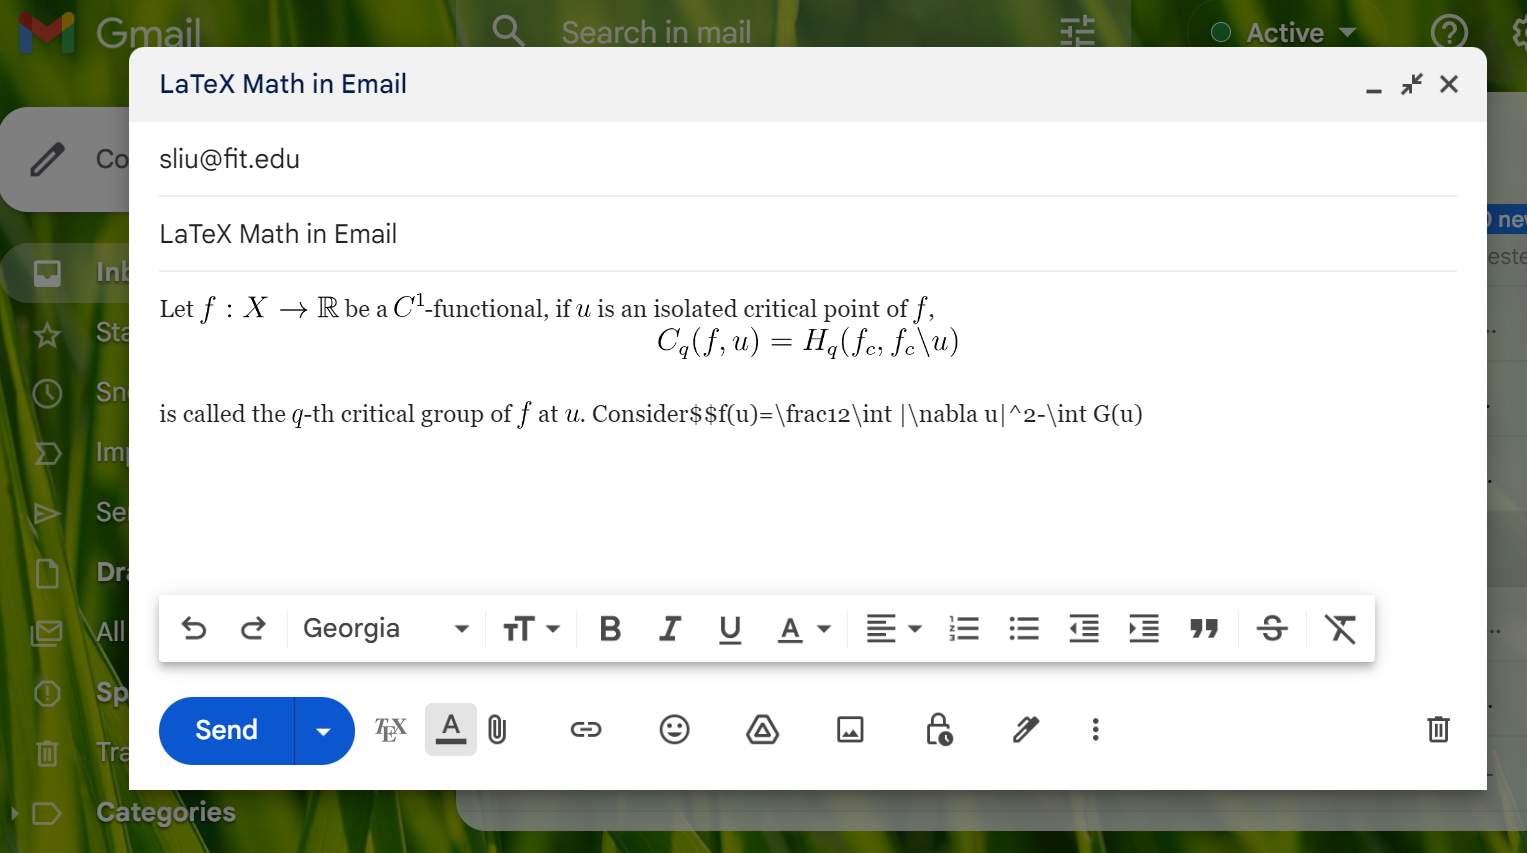
\includegraphics[width=20cm]{em-4}

\noindent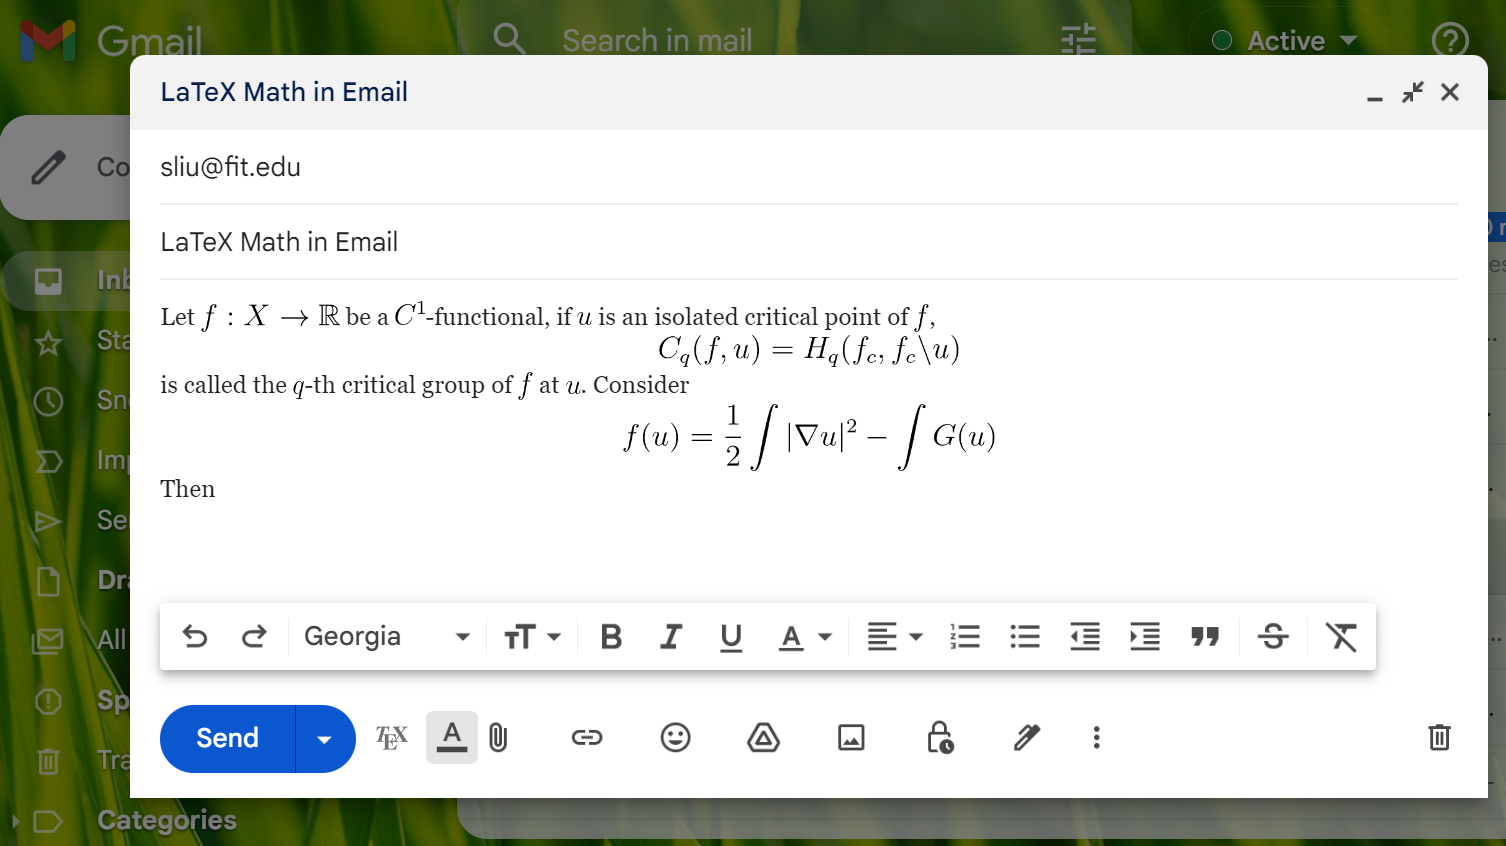
\includegraphics[width=20cm]{em-5}

\item When you have composed the email, press the Send button sending this email to the non-Gmail email address (for example \verb|sliu@fit.edu|, as shown above).
Then, login to that email account, forward the email to the desired recipient (maybe you need to deletet ``Fw'' in the Subject line, and other redundant information at the beginning of the email). The recipient will receive your email containing beautiful math formulas.

The following f{}igure shows the email with math formulas received by the third party (the desired recipient). You can see that it was sent from \verb|sliu@fit.edu|, not from Gmail.

\noindent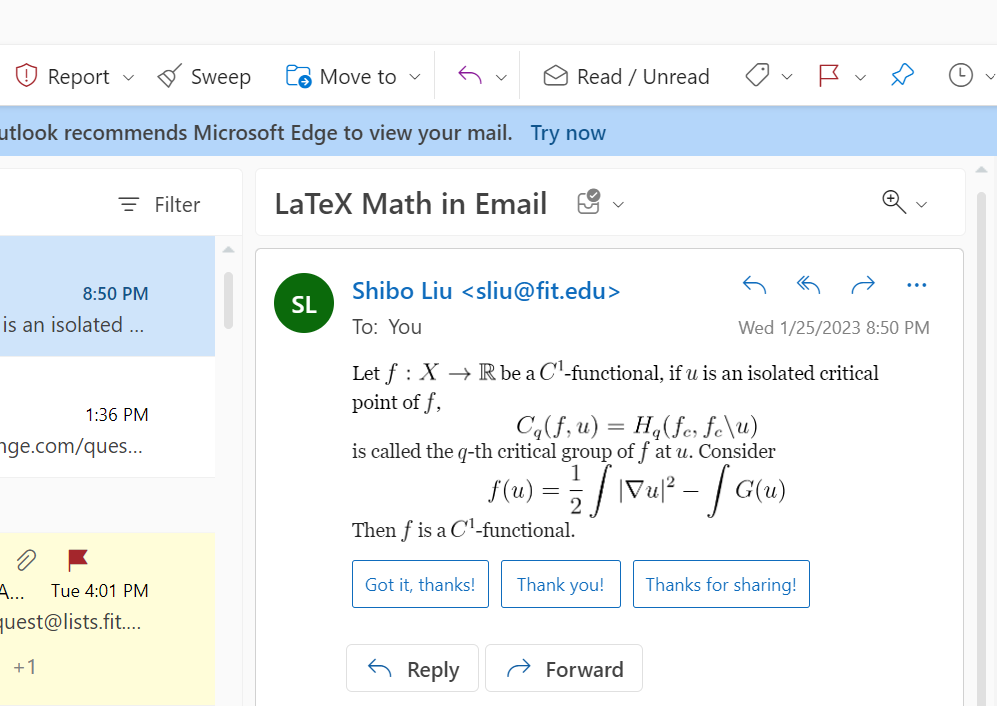
\includegraphics[width=20cm]{em-6}

\item When receiving the email, your recipient can select the text (including the math formulas and symbols) and copy + paste to a TXT editor. The \LaTeX{} codes of the math will be recovered (without the \$ or \$\$, which have to be added manually). This is another advantage of this method.

\item Some email service (such as iCloud of Apple) does not support displaying the picture of the formulas. If your recipient use this kind of email address, instead of pressing Shift + F8, you should press Shift + F9 to use the ``Simple math'' mode, which can be supported in all known email service with poorer quality:

Composing the email in Gmail (with Shift + F9), that will be sent to Apple iCloud email address:

\noindent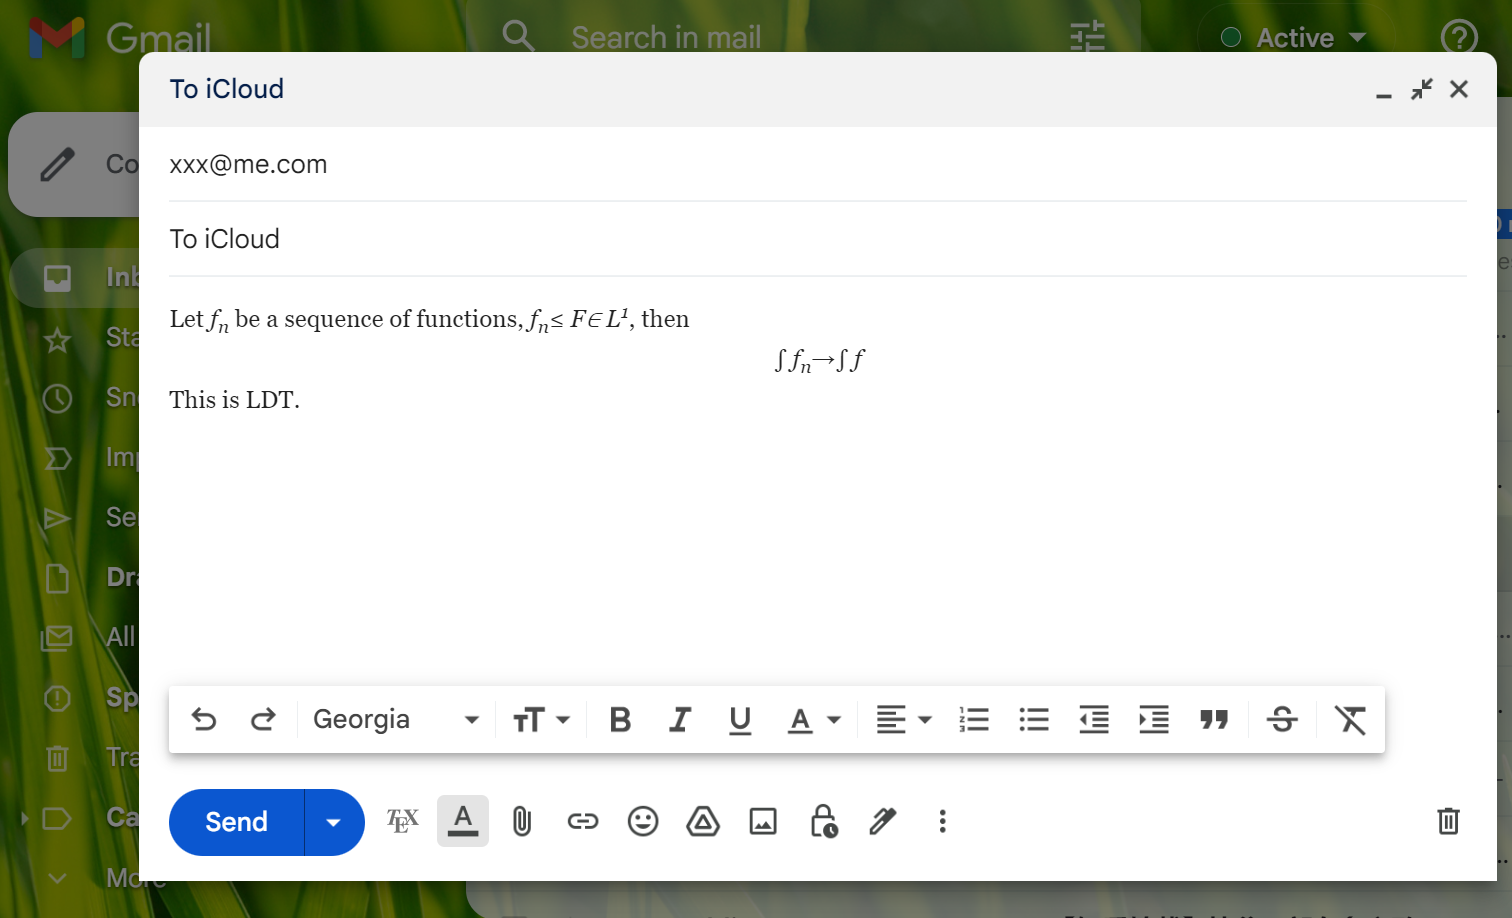
\includegraphics[width=20cm]{ei-1}

The email received in Apple iCloud email:

\noindent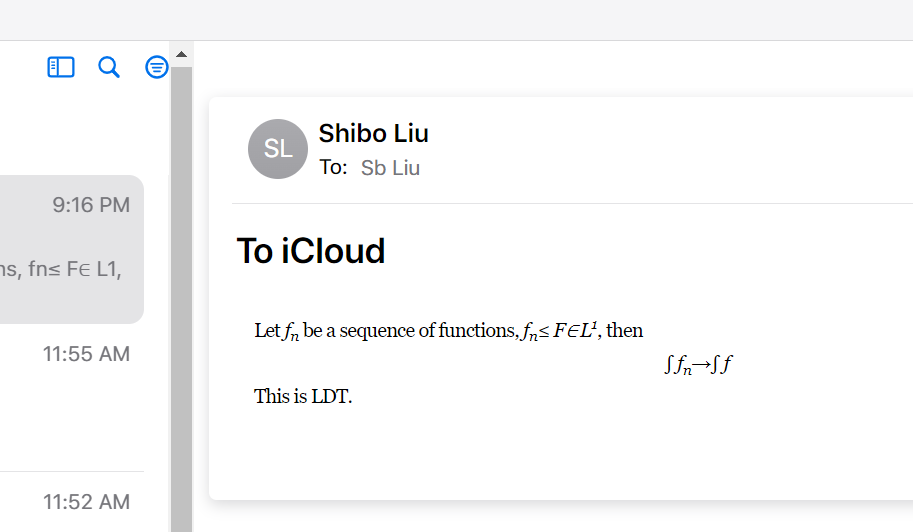
\includegraphics[width=20cm]{ei-2}

\item You can press the ``\TeX'' button near the ``Send'' button in Gmail to see what options are available.

\end{enumerate}



\end{document}
